%-----------------------------------------------------------------------------
%
%               STM paper for SYSTOR'09
%               based on: Template for LaTeX Class/Style File
%
% Template's Author: 
%               Paul C. Anagnostopoulos
%               Windfall Software
%               978 371-2316
%               paul@windfall.com
%
% Used:         31 January 2009
% Created:      15 February 2005
%
%-----------------------------------------------------------------------------


\documentclass[preprint,natbib,11pt]{sigplanconf}
% \documentclass[natbib,11pt]{sigplanconf}

\usepackage{amsmath}
\usepackage{graphicx}
\usepackage{listings}

\begin{document}

\lstset{language=C}

\conferenceinfo{SYSTOR '09}{4-6 May 2009, Haifa, Israel.} 
\copyrightyear{2009} 
\copyrightdata{[to be supplied]} 

\titlebanner{DRAFT - Do not distribute}        % These are ignored unless
\preprintfooter{STM Paper for SYSTOR}          % 'preprint' option specified.

\title{Transactifying Apache}
% \subtitle{Subtitle Text, if any}

\authorinfo{Haggai Eran\and Ohad Lutzky\and Zvika Guz\and Idit Keidar}
           {Technion}
           {haggaie@tx.technion.ac.il\and lutzky@gmail.com\and zguz@tx.technion.ac.il\and idish@ee.technion.ac.il}
%\authorinfo{Name2\and Name3}
%           {Affiliation2/3}
%           {Email2/3}

\maketitle

\begin{abstract}
Apache is a large-scale industrial multi-process and multi-threaded
application, which uses lock-based synchronization. We report on our
experience in modifying Apache to employ transactional memory instead of
locks, a process we refer to as \emph{transactification}; we are not
aware of any previous efforts to transactify legacy software of such
a large scale. Along the way, we learned some valuable lessons about
which tools one should use, which parts of the code one should
transactify and which are better left untouched, as well as on the
intricacy of commit blocks. We also stumbled across weaknesses of
existing software transactional memory (STM) toolkits, leading us
to identify desirable features they are currently lacking.
Finally, we present performance results from running
Apache on a 32-core machine, showing that, surprisingly, the performance
of the STM-based version is close to that of the lock-based version.
These results suggest that there are applications for which the overhead
of using a software-only implementation of transactional memory
is insignificant.
\end{abstract}

\category{CR-number}{subcategory}{third-level}

\terms
term1, term2

\keywords
keyword1, keyword2

\section{Introduction}

The text of the paper begins here.
\section{Related Work}
\section{Background: Software and Tools}
\subsection{Apache}
Apache\cite{apache} HTTP server is a popular web server application written in
C. It supports working on multiprocessor machines with several multi-processing
modules (MPMs) each offering a different strategy for handling requests and
distributing the work. The most popular threaded MPM is the \emph{worker} MPM,
which works by running multiple worker-threads under several processes, each
thread handles a single request at a time. In each such process there are
several worker threads, and also a listener thread that fetches incoming
requests and dispatches them to the available workers, as illustrated in Figure
~\ref{fig:apache-worker-MPM}.

\begin{figure}
 \begin{center}
  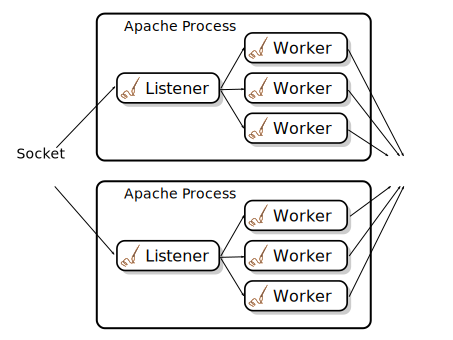
\includegraphics[width=8cm]{Apache-Worker-MPM.png}
 \end{center}
 \caption{Apache worker MPM architecture.}
 \label{fig:apache-worker-MPM}
\end{figure}

There are not many points of interaction between the worker threads themselves,
where transactional memory can be used. One such place is Apache's memory cache
implemented by the {\tt mod\_mem\_cache}\cite{apache:mod_mem_cache} module. This
module enables the workers of each process to share a cache of recently served
requests. A new request can be served from the memory cache, and save the time
required to access the disk and generate the requested page. Since the cache is
shared between multiple threads, it is synchronized by a single lock, therefore
a good candidate for converting into transactional memory.

Apache's cache is implemented with a couple of modules. The first, {\tt
mod\_cache}\cite{apache:mod_cache}, implements the logic related to caching. It
tests the metadata of each requests to see if it can be supplied from the cache,
according to the request's HTTP headers and the system configuration. It uses
one of the underlying cache implementation modules, {\tt mod\_mem\_cache} or
{\tt mod\_disk\_cache}\cite{apache:mod_disk_cache} to do the actual caching.

The {\tt mod\_mem\_cache} module implements a memory cache using a shared hash
table and priority queue. The key to the hash table is the URL of the request,
converted into a canonical form. The cache is limited both by size and by the
number of elements, and by memory size, so on insertion, sometimes lower
priority entries are removed from the cache. The priority is deterimined by one
of two algorithms: LRU, removing the least recently used entries first, and GDSF
(Greedy Dual Size Frequency) assigning score to entries based on the cost of a
cache miss, and the entry size.

\subsection{C STM Systems}
C and C++ STM systems divide into two kinds: Library based and compiler based.
Library based STMs are built as a C library. Every transaction begins with a
call into the library, and commits by another call. All reads and writes to
global variables must be done through special library functions when in a
transaction. This requires a great amount of work for converting an application
to use STM. Not only accesses to global memory in the function that started the
transaction must be converted, but also any access from any function being
called from this function. 

In contrast, compiler-based STM use a specialized compiler, which has extended
syntax for transactional memory atomic blocks. The compiler can then
automatically convert memory accesses inside transactions into calls to the
underlying library, a process sometimes referred as \emph{transactification}. 

\subsubsection{\sc Tanger}
The {\sc Tanger} ~\cite{felber2007tanger} transctifying compiler is an
open-source academic compiler extension for LLVM ~\cite{LLVM:CGO04}, an
extensible compiler framework.  Tanger aims at creating a transactifying
compiler that is independant of the STM system used. It works with the tinySTM
~\cite{felber2008tinystm} library, but can easily be extended to use other STM
libraries by writing a simple plugin.

{\sc Tanger} is accompanied with the {\sc Tarifa} ~\cite{felber2007tanger}
tool, which transactifies compiled binaries, even without the sources, which
might be a very important advantage when modifying legacy code.

\subsubsection{Intel STM Compiler}
Intel has published\cite{icc} an experimental STM compiler based on their industrial
compiler ICC. It solved the above problem by adding some new function attributes
to the language that tell the compiler which functions need to be transactified.
The attribute {\tt tm\_callable} tells the compiler that a transactified version
of the function will be needed. This way only functions that are required inside
transactions can be marked as {\tt tm\_callable} and be transactified.

Although ICC uses a proprietery STM manager, Intel has published their
ABI\cite{icc:abi} allowing for other STM managers to replace their own. This feature
and its selective transactification ability were the main reasons why we
preferred ICC.

In the latest version of Intel STM Compiler, support for abort and commit
handlers was in fact added to the system, by registering a callback function
from inside a transaction.

An extension to the Gnu Compiler Collection (GCC) is being developed\cite{gcctm} to
enable transactional memory support for GCC. It is intended to work with
tinySTM, but being open source, other STM systems will probably be ported too.
The syntax of the C/C++ language extensions is designed to be compatible with
ICC. This means that applications converted for ICC will probably be compilable
under GCC with this extension, without much modification.

\section{Transactifycation} 
\subsection{Which STM to use?}
{\sc Tanger} created a transactified version of each function in a compilation
unit.  Every function call inside a transaction was then converted to a call to
the new version. This method is a major disadvantage when working on a large
application. Many functions do not need a transactified version and this causes
uneeded work for the compiler and the linker. Moreover, sometimes the
transactifyication might fail because of calls to functions whose source is not
available and cannot be transactified. This can cause the entire build process
to fail, where in fact the code can be transactified without any error.

This was the main reason why we eventually chose to use Intel's STM Compiler.
Lately a new release of tanger was announced, one in which the developer can
annotate which functions should be transactified, however we didn't get a
chance to try it.

\subsection{What to transactify}
The conversion process included
converting critical sections protected by the cache module's main lock into
atomic blocks, and decorating required functions as {\tt tm\_callable}. The
module had used atomic instructions for some memory accesses, and these were
converted to full transactions in atomic blocks, so that collisions with these
accesses will be detected.

\subsection{Defining atomic blocks}
Some transactions, after conversion contained code that belonged with the
transactions, but didn't need neccessarily to run atomically with the
transaction. An example might be a transaction removing an object from the
cache, and freeing its memory. While the removal operation must be protected
inside a transaction, as it is using the shared memory structure of the cache,
the memory release can happen any time later, since no other thread can point to
the removed object after it had been removed from the cache. 

For lock based systems, having the memory release as part of the critical
section might cause a thread to hold the critical section a little longer than
needed, but doesn't cause any problems other than that. On transactional memory
systems, having accesses to other memory structures such as those required by
memory management might cause collisions with other threads, thus slowing down
the system in a similar way. In addition, the cleanup functions need to be
transactified, which requires additional work both from the programmer and the
compiler.

In our case, we chose not to transactify such functions, but instead remove them
from the atomic section, and execute them after the transaction had committed.
Although this requires some changes to the code, the changes are limited to the
call-site, and need not modify any of the called libraries.

For example, the following critical section in the {\tt open\_entity} function
(Figure ~\ref{code:original-open-entity}) is responsible for retrieving a page
to fullfill a request from the server. It will increment the reference count on
the cached page, and register a decrement function to be invoked upon completing
the request. When we converted the critical section into a transaction, we
didn't want the function {\tt apr\_pool\_cleanup\_register} to be called from
inside the transaction, as transactifying it would require working an another
library, the Apache Portable Runtime library, thus breaking encapsulation.

The semantics of requests and subrequest in apache guranteed the request
couldn't be completed before the return of this function, therefore we could
move the registration of the cleanup function out of the atomic section, as seen
in Figure ~\ref{code:transactified-open-entity}. However, having a commit
handler construct in the language would make such conversions easier, with it we
could register a commit handler from within the transaction, and have the STM
system automatically invoke it once the transaction had committed.

\begin{figure*}
\begin{lstlisting}
static int open_entity(cache_handle_t *h, request_rec *r, const char *key) {
  ...
  if (sconf->lock) apr_thread_mutex_lock(sconf->lock);

  obj = (cache_object_t *) cache_find(sconf->cache_cache, key);
  if (obj) {
    if (obj->complete) {
      request_rec *rmain=r, *rtmp;
      apr_atomic_inc32(&obj->refcount);
      /* cache is worried about overall counts, not 'open' ones */
      cache_update(sconf->cache_cache, obj);

      /* If this is a subrequest, register the cleanup against the main request.
       * This will prevent the cache object from being cleaned up from under the
       * request after the subrequest is destroyed. */
      rtmp = r;
      while (rtmp) {
        rmain = rtmp;
        rtmp = rmain->main;
      }
      apr_pool_cleanup_register(rmain->pool, obj, decrement_refcount, 
        apr_pool_cleanup_null);
    }
    else obj = NULL;
  }

  if (sconf->lock) apr_thread_mutex_unlock(sconf->lock);
  ...
}
\end{lstlisting}
\caption{Original {\tt open\_entity} function.}
\label{code:original-open-entity}
\end{figure*}

\begin{figure*}
\begin{lstlisting}
static int open_entity(cache_handle_t *h, request_rec *r, const char *key)
{
  ...
  __tm_atomic {
    obj = (cache_object_t *) cache_find(sconf->cache_cache, key);
    if (obj) {
      if (obj->complete) {
        ++obj->refcount;
        /* cache is worried about overall counts, not 'open' ones */
        cache_update(sconf->cache_cache, obj);
      }
      else obj = NULL;
    }
  }

  /* Register the object for removal from the cache after cleanup */
  if (obj && obj->complete) {
    request_rec *rmain=r, *rtmp;
    /* If this is a subrequest, register the cleanup against the main request.
     * This will prevent the cache object from being cleaned up from under the
     * request after the subrequest is destroyed.
     */
    rtmp = r;
    while (rtmp) {
      rmain = rtmp;
      rtmp = rmain->main;
    }
    apr_pool_cleanup_register(rmain->pool, obj, decrement_refcount, 
      apr_pool_cleanup_null);
  }
  ...
}
\end{lstlisting}
\caption{Transactified {\tt open\_entity} function.}
\label{code:transactified-open-entity}
\end{figure*}

\subsection{Commit Handlers}
Commit and undo handlers are pieces of code that are scheduled by a transaction
to run when the transaction will commit, or abort, respectively. This mechanism,
was suggested in ~\cite{tm:commit-handlers}.  Commit handlers are described
there as a mechanism that allows finalization of tasks, for instance, a
transactional system call such as write to file might have its permanent side
effects be executed in a commit handler. 
Abort handlers are called when a transaction is aborted and can reverse the 
side-effects of a transaction. These handlers can sometimes be used to implement
more efficient transactions. For example, if allocating memory inside a
transaction, (assuming without a specialized memory allocator which is available
in many STMs), the STM would need to log all the memory accesses to the memory
management data structures, and undo these writes in case of an abort. A more
efficient solution could be allocating the memory immediately, and in case of an
abort just free the memory in an abort handler.

From our perspective, commit handlers could have been used to make the
modifications we wanted in the atomic blocks, and move finalization functions
out of atomic blocks just by registering them as commit handlers. In the given
example, the call to {\tt apr\_pool\_cleanup\_register} could have been
converted into a call registering this function as a commit handler.

\section{Wish List}
\subsection{Handler Closures}
While commit handlers can aid a lot in the process of transactifying a legacy
application, their current syntax in Intel STM Compiler is very limiting.
Handlers must be given as a pointer to function of a specific signature, so a
developer trying to move a piece of code out of an atomic block, would still
need to write a new function. It would be nice to have a language construct that
defines a new commit handler right where it is being registered, however this
requires the language to support closures, and of course there are many problems
implementing those in a statically-typed language without garbage collection
such as C.

\begin{figure*}
\begin{lstlisting}
static int open_entity(cache_handle_t *h, request_rec *r, const char *key) {
  ...
  __tm_atomic {
    obj = (cache_object_t *) cache_find(sconf->cache_cache, key);
    if (obj) {
      if (obj->complete) {
        request_rec *rmain=r, *rtmp;
        ++obj->refcount;
        /* cache is worried about overall counts, not 'open' ones */
        cache_update(sconf->cache_cache, obj);

        /* If this is a subrequest, register the cleanup against the main request.
         * This will prevent the cache object from being cleaned up from under the
         * request after the subrequest is destroyed. */
        rtmp = r;
        while (rtmp) {
          rmain = rtmp;
          rtmp = rmain->main;
        }
        on_commit {
          apr_pool_cleanup_register(rmain->pool, obj, decrement_refcount, 
            apr_pool_cleanup_null);
        }
      }
      else obj = NULL;
    }
  }
  ...
}
\end{lstlisting}
\caption{{\tt open\_entity} function with a commit handler closure}
\label{code:closure-open-entity}
\end{figure*}

\subsection{Statistics and Profiling}
Intel's STM manager collects statistics about the transactions being run, their
size, abort rates, etc. Unfortunately however, it cannot work with a
multiprocess application such as Apache. This limits the ability to investigate
the performance of converted applications to only limited runs with only one
process, or having only black box measurements of the system.

\section{Evaluation} 
\subsection{Methodology} 
The transactified web server was evaluated using \emph{Siege}\cite{siege}, an
HTTP load testing tool. The server was loaded with the set of UNIX man-pages - a
set of small textual files typical of some web sites. Each page was served using
the \emph{man2html}\cite{man2html} program, uncompressed and converted into
HTML, to make sure the serving of files requires enough computational resources
to make the use of cache worthwhile.

The man2html program is a Common Gateway Interface (CGI) program that serves
unix manual (man) pages on internet sites. The pages are usually stores
compressed in gzip format, and formatted using the troff format. The program
receives a request for a man page from the webserver, uncompresses the required
file and converts it to HTML. As every CGI program it outputs the result with
relevant HTTP headers.

The default caching policy of apache forbids caching dynamically generated pages
such as those of man2html, unless the HTTP headers of the resulting page clearly
specify otherwise. To make caching of the man2html pages possible, we modified
man2html to output such headers, specifying the output can be cached for one
hour.

The pages were requested randomly according to Zipf distribution, whose
parameter $s$ determines how frequently the most popular pages were visited,
thus controlling the amount of locality in the requests.

The experiments were done with two computers connected using Gigabit ethernet.
The machine running the server was a 4 processors SMP of dual core 2.66GHz Xeons
with 8GB of RAM, and the client machine was a 2 processors SMP of quad core
2.33Ghz E5410 Xeons with 8GB of RAM. [TBD: Update to neo and trinity]

\subsection{Results} 
We compared the average latency and request throughput when running on different
number of cores, and with different  values. For every graph there are three
experiments comparing the results of an Apache server running without a cache, a
cached version without our transactional modifications, and the transactified
version. 

\begin{figure}
 \begin{center}
  \includegraphics[width=8cm]{transaction-rate-single-host-1.png}
 \end{center}
 \caption{Transaction Rate, Single host, $s = 1$}
 \label{fig:transaction-rate-single-host-1}
\end{figure}
\begin{figure}
 \begin{center}
  %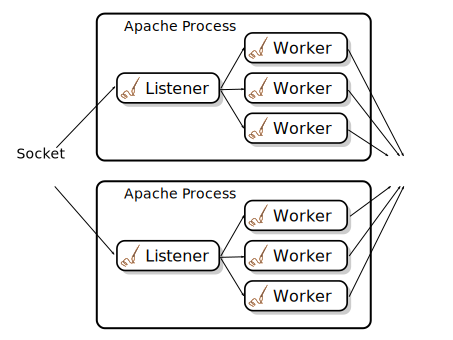
\includegraphics[width=8cm]{Apache-Worker-MPM.png}
 \end{center}
 \caption{Average Response Time, $s = 1$}
 \label{fig:response-time-1}
\end{figure}
\begin{figure}
 \begin{center}
  %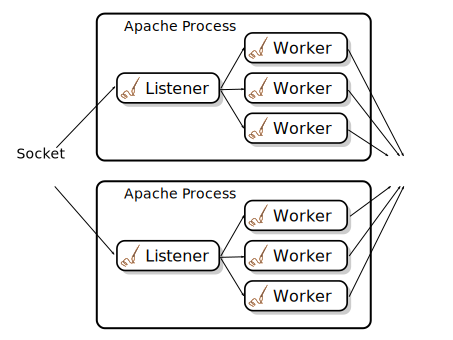
\includegraphics[width=8cm]{Apache-Worker-MPM.png}
 \end{center}
 \caption{Average Response Time, $s = 2$}
 \label{fig:response-time-2}
\end{figure}
\begin{figure}
 \begin{center}
  %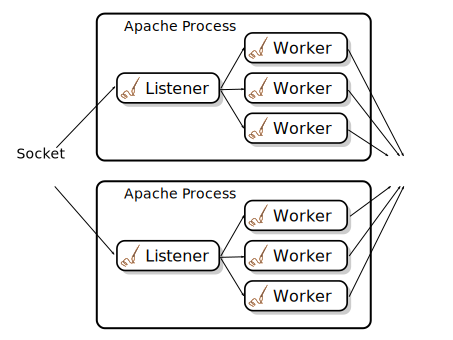
\includegraphics[width=8cm]{Apache-Worker-MPM.png}
 \end{center}
 \caption{Transaction Rate, $s = 1$}
 \label{fig:transaction-rate-1}
\end{figure}
\begin{figure}
 \begin{center}
  %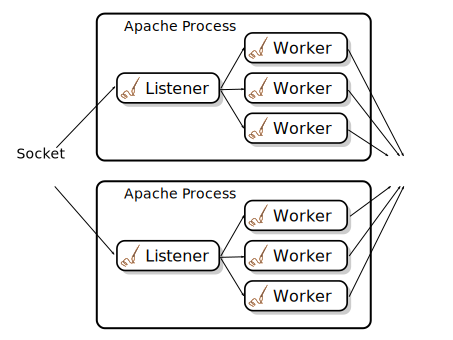
\includegraphics[width=8cm]{Apache-Worker-MPM.png}
 \end{center}
 \caption{Transaction Rate, $s = 2$}
 \label{fig:transaction-rate-2}
\end{figure}
\begin{figure}
 \begin{center}
  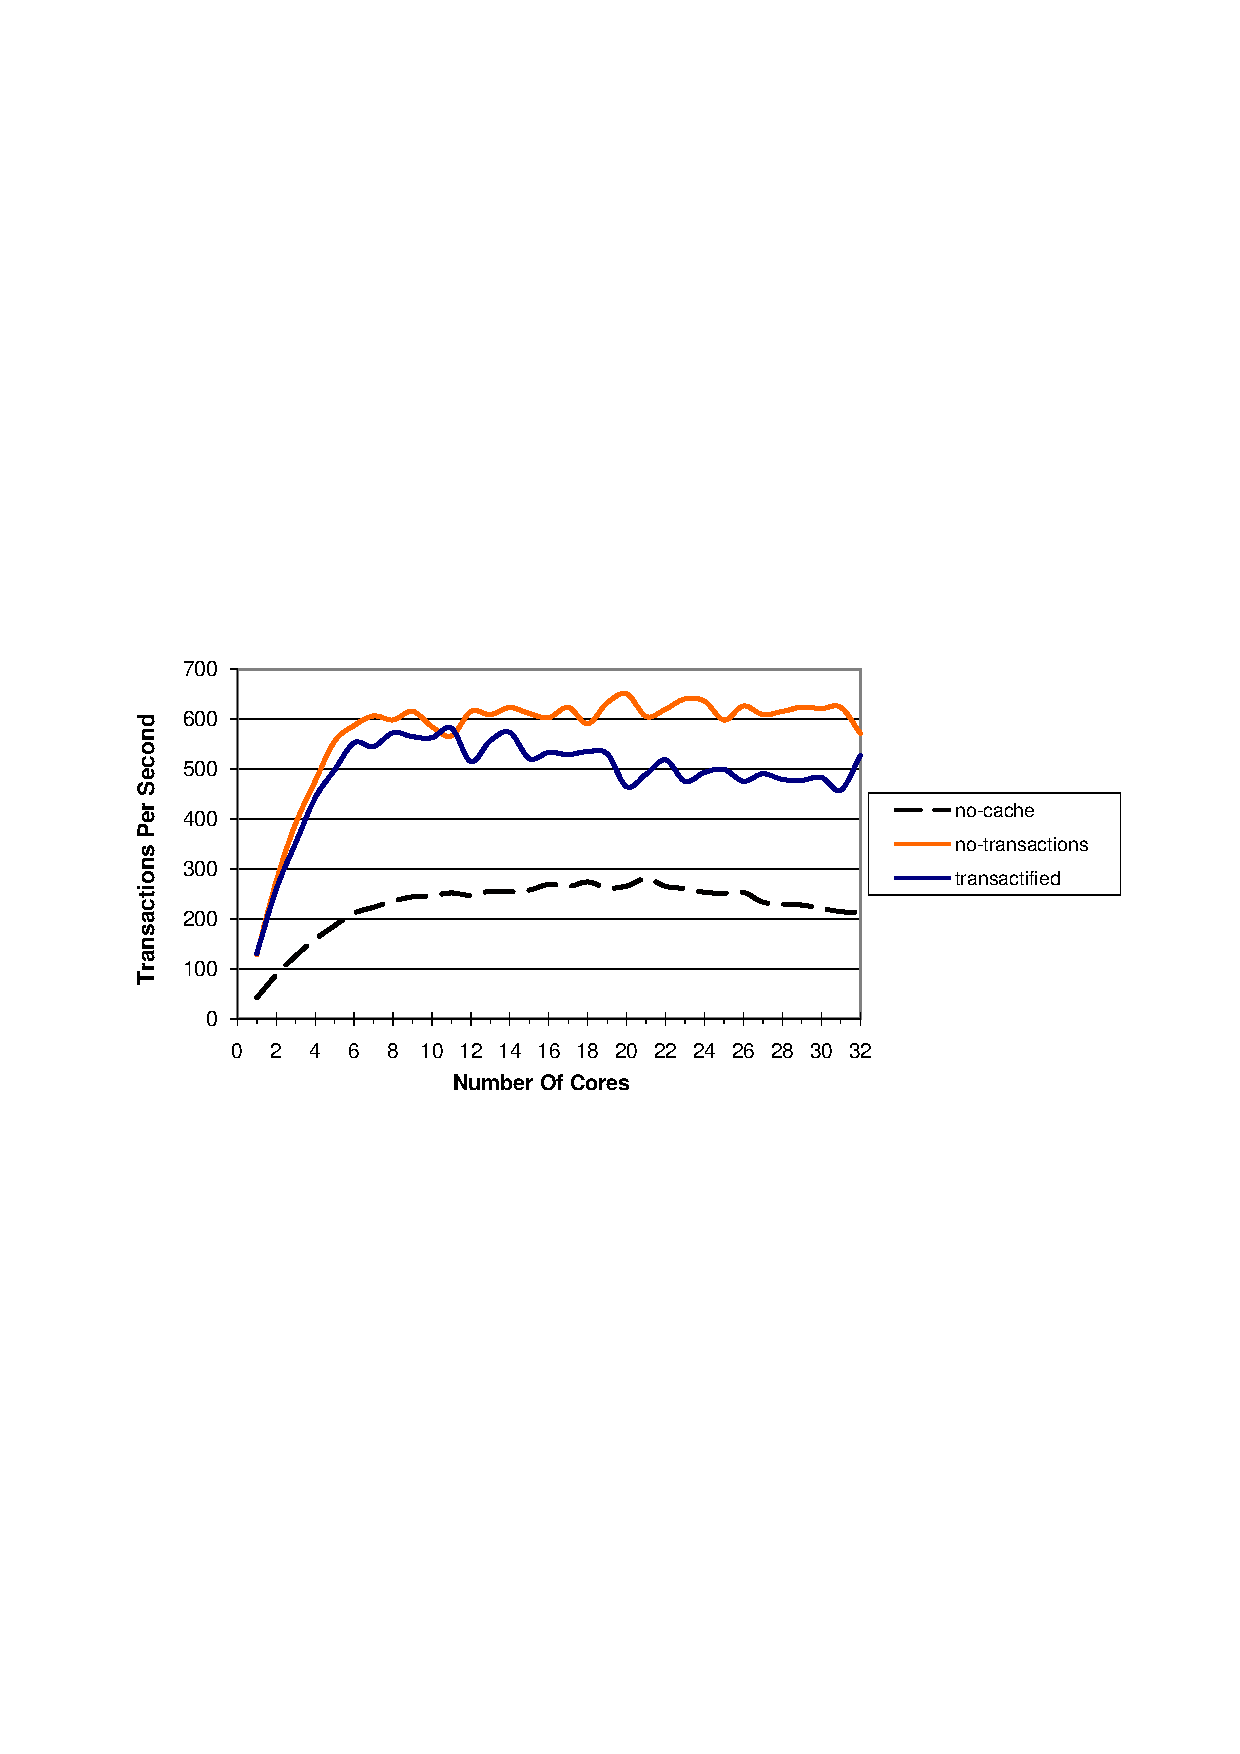
\includegraphics[width=8cm]{transaction-rate-single-process.png}
 \end{center}
 \caption{Transaction Rate, $s = 1$, a single process}
 \label{fig:one-process-transaction-rate}
\end{figure}
\begin{figure}
 \begin{center}
  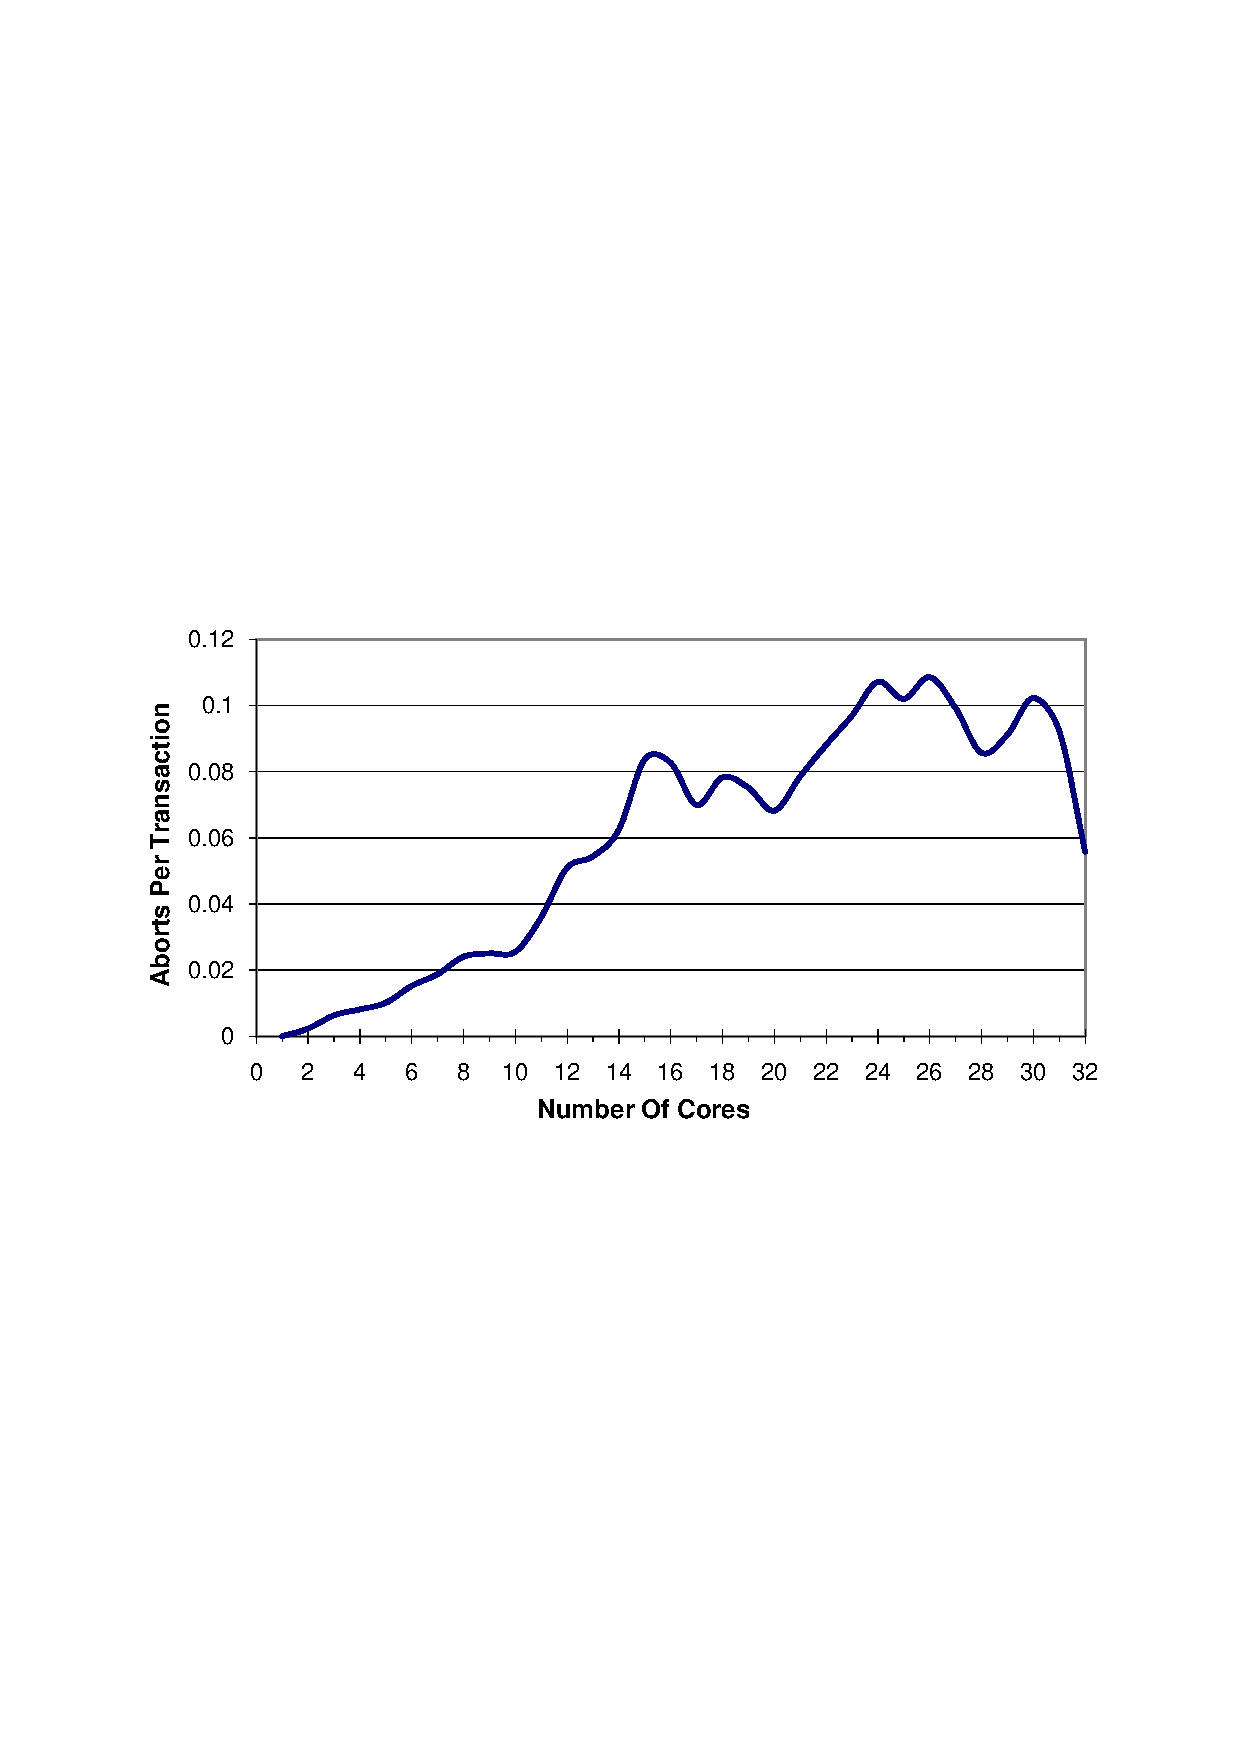
\includegraphics[width=8cm]{abort-rate.png}
 \end{center}
 \caption{Abort Rate, $s = 1$, a single process}
 \label{fig:abort-rate}
\end{figure}

\section{Conclusions}
\begin{itemize}
  \item Out of 340,000 lines of code in the Apache Web server, the cache module is comprised of only 6651 lines of code, of which only 273 lines were changed by our modifications. This shows the importance of being able to modify only encapsulated sections of the code, and interoperating with legacy code that still uses locks.  
  \item Having commit handlers in the STM system is not only needed for creating efficient open transactions, but can also aid the process of transactifying legacy code.
  \item There is great importance in working on real-world applications as they may reveal challenges resulting from engineering problems and not only algorithmic and theoretical problems.
\end{itemize}
There are many STM systems currently available, and one immediate direction would be to compare them using this benchmark. This would require writing plugins for any such system to match Intel's TM ABI. 

In addition, there are other applications that might be interesting as transactional memory applications, following the methods we used.

\appendix
\section{Appendix Title}

This is the text of the appendix, if you need one.

\acks

Acknowledgments, if needed.

\bibliographystyle{plainnat}

%\begin{thebibliography}{}
%
%\bibitem{smith02}
%Smith, P. Q. reference text
%
%\end{thebibliography}

\bibliography{references}

\end{document}

